\documentclass[24pt]{beamer}
\usepackage[utf8]{inputenc}
\usepackage[utf8]{vietnam}
\usepackage{amsmath}
\usepackage{amsfonts}
\usepackage{amssymb}
\usepackage{graphicx}
\usepackage{tikz}
\usetikzlibrary{positioning}
\usepackage{xcolor}
\usepackage{utopia} %font utopia imported
\usepackage{siunitx}
\usepackage[american,cuteinductors,smartlabels]{circuitikz}
\usepackage{ragged2e}
\usepackage{etoolbox}

\mode<beamer>{\usetheme{CambridgeUS}}

\usecolortheme{default}

\usepackage{hyperref}
\hypersetup{pdfpagemode=FullScreen} %mode FullScreen with beamer

\apptocmd{\frame}{}{\justifying}{} % Allow optional arguments after frame.

\usepackage{comment}

\makeatletter
\let\insertuniversity\relax
\newcommand\universitytitle{TRƯỜNG ĐH}

\let\insertclass\relax
\newcommand\classtitle{Lớp}

\let\insertcourse\relax
\newcommand\coursetitle{Môn học}

\mode<all>
{
  \newcommand\university[1]{\def\insertuniversity{#1}}
  
  \newcommand\class[1]{\def\insertclass{#1}}
  
  \newcommand\course[1]{\def\insertcourse{#1}}
  \titlegraphic{}
}

\defbeamertemplate*{title page}{supdefault}[1][]
{
  \begingroup
    \centering
    \ifx\insertuniversity\relax\relax\else
    \begin{beamercolorbox}[sep=2pt,center,#1]{author}
      \hspace{-.15cm}\scriptsize\universitytitle~\insertuniversity
    \end{beamercolorbox}\fi
    
    \begin{beamercolorbox}[sep=8pt,center,#1]{title}
      \usebeamerfont{title}\normalsize\inserttitle\par%
      \ifx\insertsubtitle\@empty\relax%
      \else%
        \vskip0.25em%
        {\usebeamerfont{subtitle}\usebeamercolor[fg]{subtitle}\insertsubtitle\par}%
      \fi%     
    \end{beamercolorbox}%
    \vskip.5em\par

    \vspace{-.4cm}
    \ifx\insertcourse\relax\relax\else
    \begin{beamercolorbox}[sep=6pt,center,#1]{author}
      \usebeamerfont{author}\footnotesize\coursetitle:~\insertcourse
    \end{beamercolorbox}\fi

    \vspace{-.3cm}
    \ifx\insertclass\relax\relax\else
    \begin{beamercolorbox}[sep=6pt,center,#1]{author}
      \usebeamerfont{author}\footnotesize\classtitle:~\insertclass
    \end{beamercolorbox}\fi

    \vspace{-.3cm}
    \begin{beamercolorbox}[sep=6pt,center,#1]{author}
      \usebeamerfont{author}\hspace{-.23cm}\footnotesize\insertauthor
    \end{beamercolorbox}
    %\begin{beamercolorbox}[sep=8pt,center,#1]{institute}
      %\usebeamerfont{institute}\insertinstitute
    %\end{beamercolorbox}
    \vspace{-.4cm}
    \begin{beamercolorbox}[sep=8pt,center,#1]{date}
      \usebeamerfont{date}\footnotesize\insertdate
    \end{beamercolorbox}\vskip0.5em
    {\usebeamercolor[fg]{titlegraphic}\inserttitlegraphic\par}
  \endgroup
  \vfill
}
\setbeamertemplate{title page}[supdefault][colsep=-4bp,rounded=true,shadow=\beamer@themerounded@shadow]\makeatother

%Title page
\title[Động cơ không đồng bộ]{\emph{Chủ đề báo cáo}\\ ĐK Công suất trượt về nguồn và ĐK ĐC dùng biến tần}
\author[Cơ sở Truyền động điện]{GVHD: Hồ Minh Nhị \and Nhóm SVTH: Nhóm 1}
\course{Cơ sở Truyền động điện}
\class{Công nghệ, kỹ thuật điện, điện tử}
\university{KỸ THUẬT -- CÔNG NGHỆ CẦN THƠ}
\date[Nhóm 1]{\today}
%\date[Nhóm 1]{Ngày 24 tháng 08 năm 2016}

%\logo{
\includegraphics[height=1.3cm]{logo_ctut.pdf}}

\AtBeginSection[]
{
  \begin{frame}
    \frametitle{Nội dung báo cáo}
    \justifying
    \tableofcontents[currentsection]
  \end{frame}
}
\definecolor{doden}{RGB}{204, 0, 0}
\newcommand{\noibat}[1]{\textcolor{red}{#1}}
\begin{document}
%http://tex.stackexchange.com/questions/82794/removing-page-number-from-title-frame-without-changing-the-theme
\bgroup
\makeatletter
\setbeamertemplate{footline}
{
  \leavevmode%
  \hbox{%
  \begin{beamercolorbox}[wd=.333333\paperwidth,ht=2.25ex,dp=1ex,center]{author in head/foot}%
    \usebeamerfont{author in head/foot}\insertshortauthor\expandafter\beamer@ifempty\expandafter{\beamer@shortinstitute}{}{~~(\insertshortinstitute)}
  \end{beamercolorbox}%
  \begin{beamercolorbox}[wd=.333333\paperwidth,ht=2.25ex,dp=1ex,center]{title in head/foot}%
    \usebeamerfont{title in head/foot}\insertshorttitle
  \end{beamercolorbox}%
  \begin{beamercolorbox}[wd=.333333\paperwidth,ht=2.25ex,dp=1ex,right]{date in head/foot}%
    \usebeamerfont{date in head/foot}\insertshortdate{}\hspace*{2em}
%    \insertframenumber{} / \inserttotalframenumber\hspace*{2ex} 
    \hspace*{6ex}
  \end{beamercolorbox}}%
  \vskip0pt%
}

\begin{frame}
\titlepage
\end{frame}
\egroup

\setcounter{framenumber}{0}

%--------------------------------------------------------------------------------
%--------------------------------------------------------------------------------
% Danh sach thanh vien
\begin{frame}{Danh sách thành viên}
%	\vspace{-1cm}
	\begin{footnotesize}
	\begin{columns}
		\column{0.6\textwidth}
		\begin{enumerate}
			\item Nguyễn Văn Bảy
			\item Nguyễn Văn Đình
			\item Nguyễn Hoàng Hận
			\item Thi Minh Nhựt
			\item Phạm Thanh Quý
			\item Hồ Minh Thành
			\end{enumerate}

		\column{.6\textwidth}
		\begin{enumerate}	% Danh sach tiep theo
			\setcounter{enumi}{6}
			\item Nguyễn Văn Tiến
			\item Liên Thái Trường
			\item Trần Thanh Tú
			\item Bùi Trọng Tuấn
			\item Lư Anh Tuấn
			\item Nguyễn Bá Vọng
		\end{enumerate}
	\end{columns}
	\end{footnotesize}
\end{frame}

%--------------------------------------------------------------------------------
%--------------------------------------------------------------------------------
% Noi dung bao cao
\begin	{frame}	%Trang muc luc
	\frametitle{Nội dung báo cáo}
	\tableofcontents
\end{frame}
%--------------------------------------------------------------------------------
%--------------------------------------------------------------------------------
\section[Công suất trượt]{Điều khiển công suất trượt trả về nguồn}
\subsection*{Phạm vi áp dụng}
\begin{frame}{ĐK công suất trượt}
	\begin{block}{Phạm vi áp dụng}
		\begin{itemize}
			\justifying
			\item ĐC KĐB roto dây quấn công suất lớn.
			\item ĐK được tốc độ dưới đồng bộ và trên đồng bộ.
		\end{itemize}				
	\end{block}
\end{frame}

\subsection*{Nguyên tắc biến đổi}
\begin{frame}{ĐK công suất trượt}
\begin{block}{Nguyên tắc biến đổi}
		\begin{itemize}
		\justifying
		\item Năng lượng ở mạch rotor qua bộ biến đổi công suất trả về nguồn xoay chiều.
		\item ĐK $P_r \longrightarrow$ ĐK $M, n$ của ĐC.
		\end{itemize}
	\end{block}
\end{frame}

\subsection*{Nguyên tắc hoạt động}
\begin{frame}{ĐK công suất trượt}
\begin{block}{Nguyên tắc hoạt động}
		\begin{itemize}
		\justifying
		\item Đưa vào rotor sức điện động phụ cùng tần số với rotor.
		\item Sức điện động: nguồn $AC$ hoặc $DC$.
		\end{itemize}
	\end{block}
\end{frame}

\subsection*{ĐK dưới vận tốc đồng bộ}
\begin{frame}{ĐK công suất trượt}
		\begin{center}
			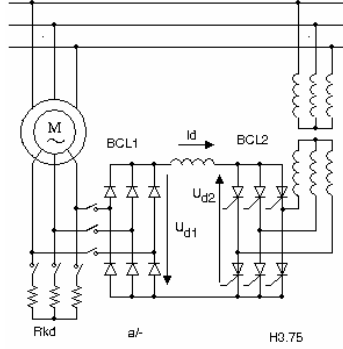
\includegraphics[scale=.5]{images-chude3/cascade-2.png} 
		\end{center}
\end{frame}

\subsection*{ĐK trên vận tốc đồng bộ}
\begin{frame}{ĐK công suất trượt}
		\begin{center}
			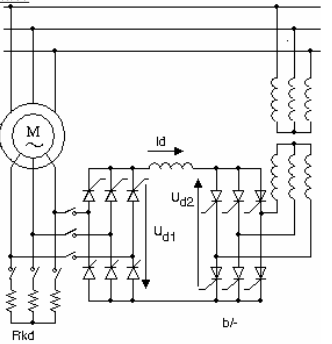
\includegraphics[scale=.5]{images-chude3/cascade.png} 
		\end{center}
\end{frame}

\subsection*{Ưu và nhược điểm}
\begin{frame}{ĐK công suất trượt}
\begin{block}{Ưu điểm}
\justifying
		Tận dụng được công suất trượt ở mạch rotor.
	\end{block}
\end{frame}

\begin{frame}{ĐK công suất trượt}
	\begin{block}{Nhược điểm}
		\begin{itemize}
		\justifying
			\item Mạch điều khiển và mạch động lực phức tạp.
			\item Phạm vi điều khiển tốc độ không lớn, moment giảm.
		\end{itemize}
	\end{block}
\end{frame}
%--------------------------------------------------------------------------------
%--------------------------------------------------------------------------------
\section[Biến tần]{Điều khiển động cơ dùng biến tần}
\subsection*{Khái quát}
\begin{frame}{Khái quát biến tần}
	\begin{block}{Chức năng}	
		$U_1, I_1, f_1 \longrightarrow U_2, I_2, f_2$
	\end{block}
	
	\begin{block}{Ứng dụng}	
	\justifying
		Điều khiển \noibat{tốc độ} ĐC. Thay đổi được \noibat{số pha}.
	\end{block}
\end{frame}

\begin{frame}{Khái quát biến tần}
	\begin{block}{Phân loại}
		\begin{itemize}
		\justifying
			\item Theo \textcolor{blue}{số pha}: \noibat{$1$ pha}, \noibat{$3$ pha}, $m$ pha.
			\item Theo \textcolor{blue}{cấu trúc}: biến tần \noibat{trực tiếp} và biến tần \noibat{gián tiếp}.
		\end{itemize}
	\end{block}
\end{frame}

\subsection*{Cấu tạo}
\begin{frame}{Cấu tạo biến tần}
	\vspace{-2cm}
	\begin{flushleft}
		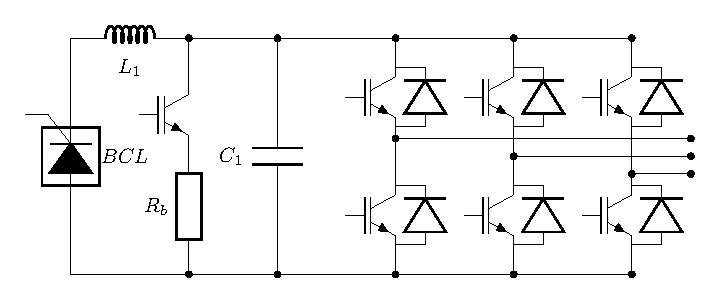
\includegraphics[scale=1]{images-chude3/bientan.pdf}
	\end{flushleft}
\end{frame}

\begin{frame}{Cấu tạo biến tần}
	\begin{itemize}
		\item Bộ chỉnh lưu.
		\item Mạch trung gian (nếu có).
		\item Bộ nghịch lưu.
	\end{itemize}
	\begin{block}{Nguyên lý hoạt động}
		$AC \longrightarrow DC \longrightarrow AC$
	\end{block}
\end{frame}

\subsection*{Ưu điểm}
\begin{frame}{Ưu điểm}
	\begin{block}{Ưu điểm}
		\begin{itemize}	
		\justifying
			\item Điều khiển tốc độ động cơ dễ dàng.
			\item Tiết kiệm năng lượng.
			\item Tăng tuổi thọ cho động cơ.
		\end{itemize}
	\end{block}
\end{frame}


%--------------------------------------------------------------------------------
%--------------------------------------------------------------------------------
% Tai lieu tham khao
\section*{Tài liệu tham khảo}
\begin{frame}{Tài liệu tham khảo}
\begin{small}
\justifying
[1]. Nguyễn Văn Nhờ, \textit{Cơ sở Truyền động điện}, NXB ĐH Quốc gia HCM.

[2]. Nguyễn Văn Nhờ, \textit{Điện tử công suất 1}, NXB ĐH Quốc gia HCM.
\end{small}
\end{frame}
%https://2bientan.wordpress.com/2015/03/31/khoi-dong-mem-la-gi-tai-lieu-va-nguyen-ly-khoi-dong-mem/
%--------------------------------------------------------------------------------
%--------------------------------------------------------------------------------
% Lời cảm ơn
\section*{Lời cảm ơn}
\begin{frame}
\justifying
\large \alert{Cảm ơn Thầy và các bạn đã quan tâm theo dõi phần trình bày của nhóm!}
\end{frame}
\end{document}